%
% hauptkruemmungen.tex
%
% (c) 2017 Prof Dr Andreas Müller, Hochschule Rapperswil
%
\section{Hauptkrümmungen}
\rhead{Hauptkrümmungen}
In Abschnitt~\eqref{skript:kruemmung:richtungsabhaengigkeit} wurde gezeigt,
dass die Schnittkrümmungen $\kappa(e)$ in Abhängigkeit von der
Tangentenrichtung $e$ dank der Wahl eines speziellen Koordinatensystems
mit Hilfe der Matrix der zweiten Ableitung berechnet werden kann.
Wenn $e$ ein Einheitsvektor ist, dann haben wir gefunden, dass die
Schnittkrümmung
\[
\kappa(e)
=
2\biggl(
\frac{\partial^2 f}{\partial x^2}
e_1^2
+
2
\frac{\partial^2 f}{\partial x\partial y}e_1e_2
+
\frac{\partial^2 f}{\partial y^2}e_2^2
\biggr)
\]
ist.
In dieser Form ist nicht klar erkennbar, wie $\kappa(e)$ von $e$ abhängt.

Wir können $\kappa(e)$ aber auch in Vektorform schreiben.
Dazu schreiben wir die Matrix der zweiten Ableitungen als
\[
H
=
\begin{pmatrix}
\displaystyle\frac{\partial^2 f}{\partial x^2}&
\displaystyle\frac{\partial^2 f}{\partial x\partial y}\\
\displaystyle\frac{\partial^2 f}{\partial x\partial y}&
\displaystyle\frac{\partial^2 f}{\partial y^2}
\end{pmatrix},
\]
sie heisst die {\em Hessische Matrix}.
Damit kann die Krümmung als Matrizenprodukt geschrieben werden:
\[
\kappa(e)
=
\begin{pmatrix}e_1&e_2\end{pmatrix}
\begin{pmatrix}
\displaystyle\frac{\partial^2 f}{\partial x^2}&
\displaystyle\frac{\partial^2 f}{\partial x\partial y}\\
\displaystyle\frac{\partial^2 f}{\partial x\partial y}&
\displaystyle\frac{\partial^2 f}{\partial y^2}
\end{pmatrix}
\begin{pmatrix}e_1\\e_2\end{pmatrix}
=
e^tHe.
\]
Die Matrix $H$ ist offenbar symmetrisch.

\begin{figure}
\centering
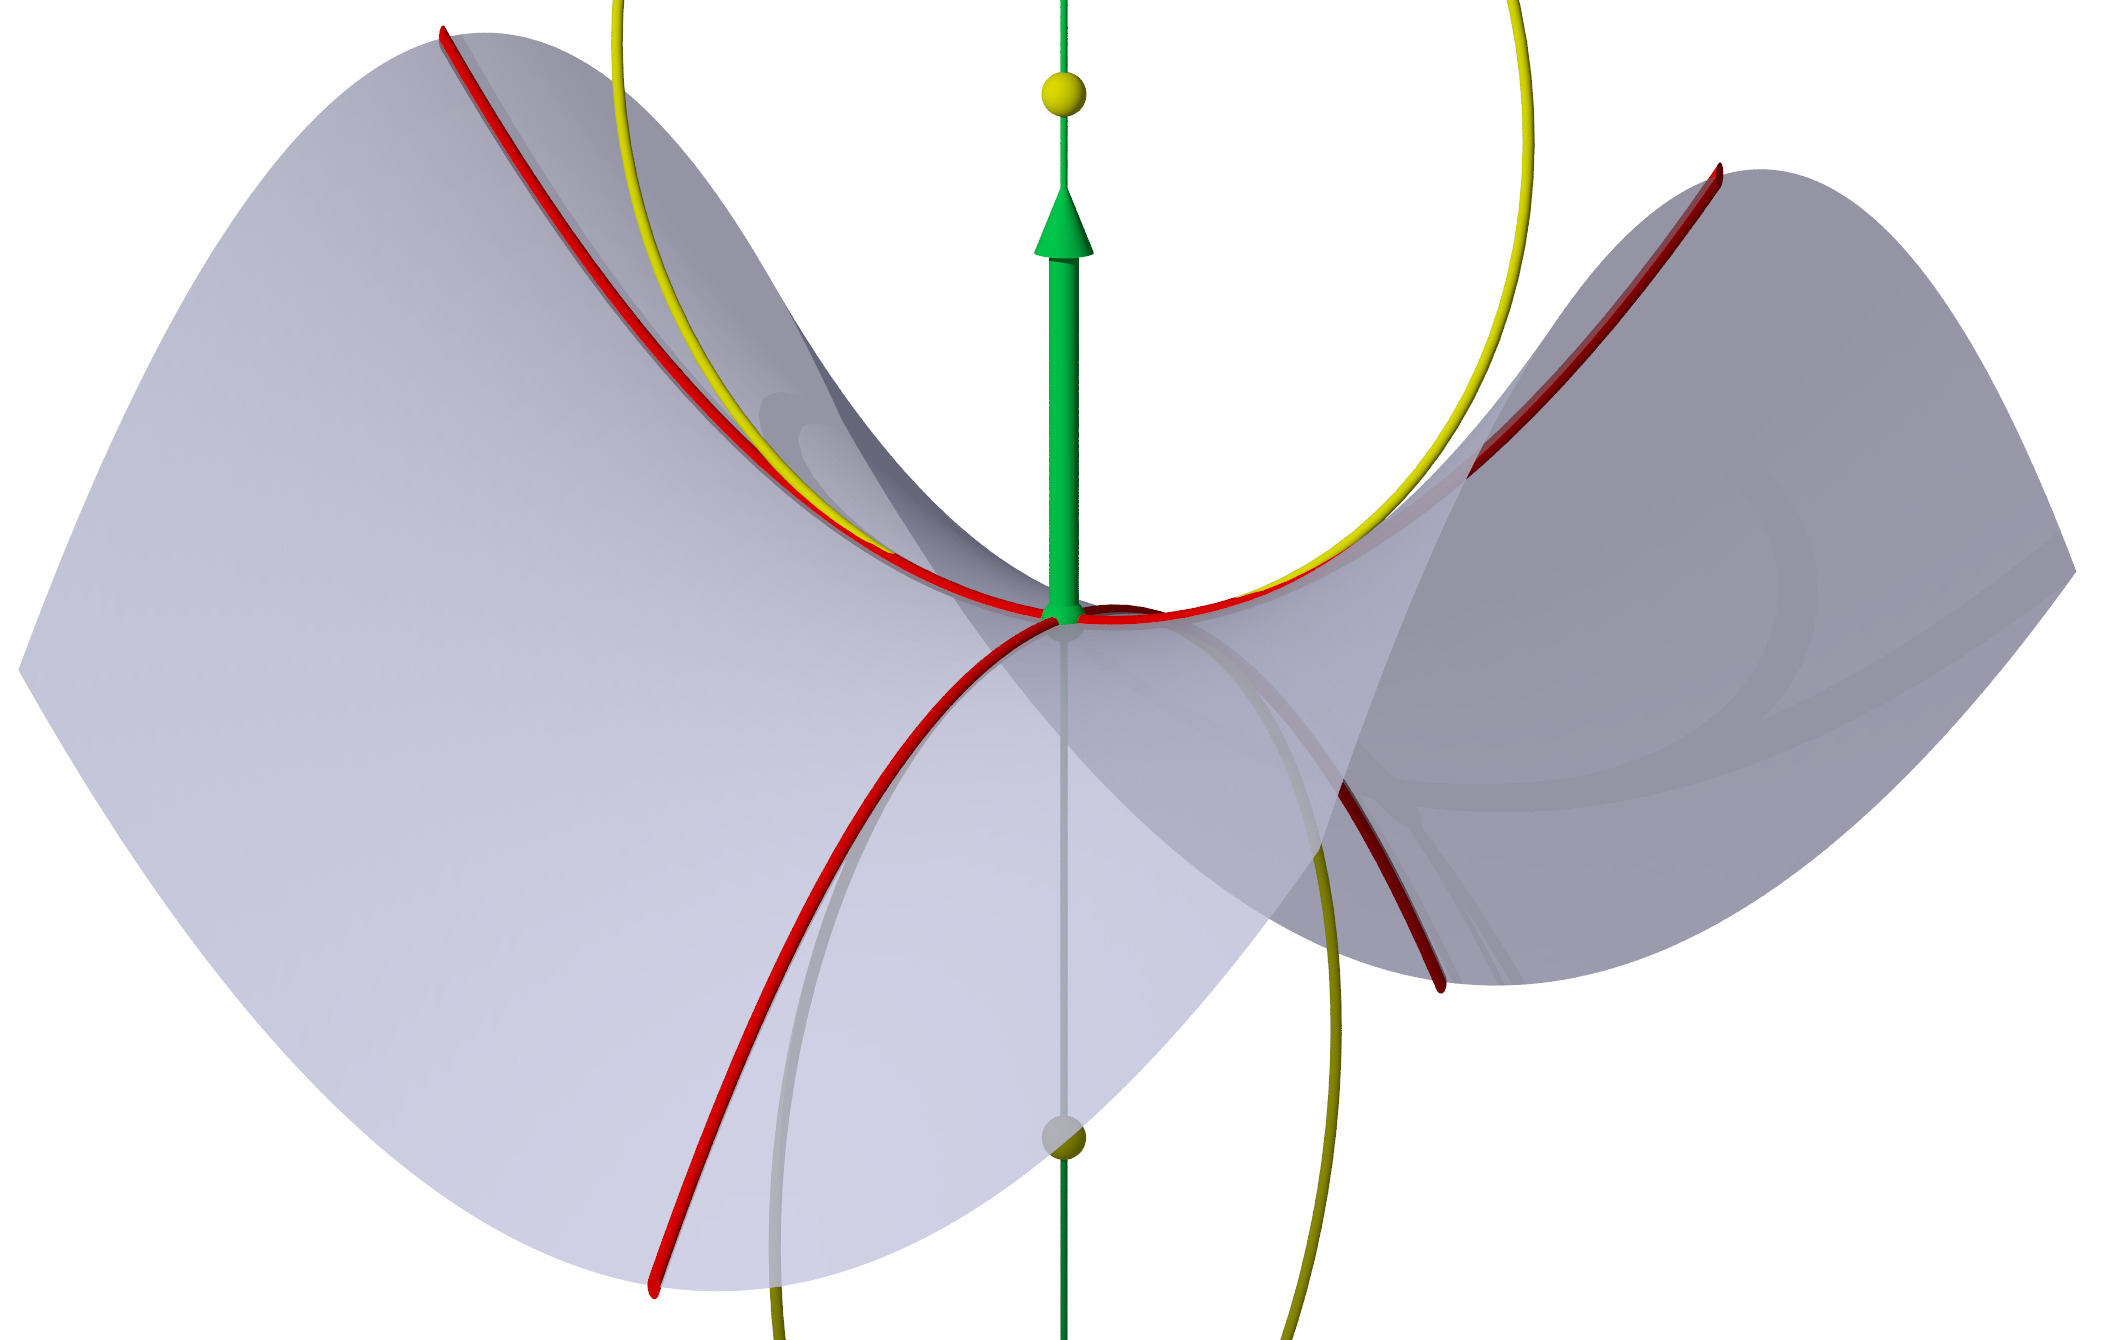
\includegraphics[width=\hsize]{chapters/3d/hauptkruemmungen.jpg}
\caption{Die Hauptkrümmungen einer Fläche sind die maximale und minimale
Schnittkrümmung in einem Punkte.
Die zugehörigen Krümmungsrichtungen heissen die Hauptkrümmungsrichtungen.
In diesem Beispiel haben die beiden Hauptkrümmungen verschiedenes Vorzeichen.
\label{skript:kurven:hauptkruemmungen}}
\end{figure}

In der linearen Algebra lernt man, dass sich jede symmetrische Matrix 
mit Hilfe einer Matrix in $\textrm{SO}(n)$ diagonalisieren lässt.
Im vorliegenden Fall gibt es eine Drehung der $x$-$y$-Ebene derart, dass
die Matrix $H$ Diagonalform bekommt.
Die Krümmung in Abhängigkeit vom Einheitsvektor $e$ ist daher
\[
\kappa(e)
=
2\lambda_1 e_1^2 + 2\lambda_2 e_2^2,
\]
wobei $\lambda_1$ und $\lambda_2$ die Eigenwerte von $H$ sind.
Für $e_1=\cos\alpha$ und $e_2=\sin\alpha$ bekommt man
\[
\kappa(\alpha)
=
2\lambda_1 \cos^2\alpha + 2\lambda_2 \sin^2\alpha.
\]
Diese Funktion nimmt ihr Maximum und Minimum auf den Achsen an,
die Eigenwerte sind also bis auf den Faktor $2$ die maximale und minimale
Schnittkrümmung.
Wir schreiben $\kappa_1=2\lambda_1$ und $\kappa_2=2\lambda_2$ für die
beiden zugehörigen Krümmungen.
\index{Hauptkrümmungen}
Diese heissen auch die Hauptkrümmungen, die Richtungen der Achsen heissen
die Hauptkrümmungsrichtung, und sie stehen senkrecht aufeinander, weil
\index{Hauptkrümmungsrichtung}
die Eigenvektoren einer symmetrischen Matrix zu verschiedenen Eigenvektoren
immer senkrecht aufeinander stehen.

\subsection{Invarianten}
Die hessische Matrix $H$ hat die Eigenwerte $\lambda_1$ und $\lambda_2$.
Diese sind für sich genommen nicht interessant.
Hingegen sind die Determinante und die Spur von $H$ Invarianten, die
unabhängig von der Richtung der Achsen in der $x$-$y$-Ebene sind.

\subsubsection{Determinante -- Gausskrümmung}
\index{Gausskrümmung}
\index{Krümmung!Gauss-}
Die Determinante von $H$ ist das Produkt der Eigenwerte, also
\[
\det H
=
\lambda_1\lambda_2
=
\frac14 (2\lambda_1) (2\lambda_2)
=
\frac14 \kappa_1\kappa_2.
\]
\begin{definition}
\label{skript:definition:gausskruemmung}
Das Produkt der Hauptkrümmungen $K=\kappa_1\kappa_2$
heisst {\em Gausskrümmung} der Fläche.
\end{definition}
Es stellt sich heraus, dass die Gausskrümmung auch aus inneren Eigenschaften
der Fläche ermittelt werden kann
(Theorema Egregium von Gauss).
Wir werden in Kapitel~\ref{skript:chapter:kruemmung} 
mit der Riemannsschen Krümmung ein Konzept der Krümmung eines Raumes
definieren, welches für Flächen im Wesentlichen mit der Gausskrümmung
übereinstimmt.

\subsubsection{Spur -- mittlere Krümmung}
\index{mittlere Krümmung}
\index{Krümmung!mittlere}
Die Spur von $H$ ist eine weitere Invariante der Matrix.
Es gilt
\[
\operatorname{Spur} H
=
\lambda_1+\lambda_2
=
\frac12(2\lambda_1+2\lambda_2)
=
\frac12(\kappa_1+\kappa_2).
\]
In Abschnitt~\ref{skript:kurve:mittlerekruemmung} haben wir nachgeweisen,
dass die mittlere Krümmung gleichzeitig die Spur der Hessischen Matrix ist.
Obige Überlegung zeigt, dass dies auch der Mittelwert der Hauptkrümmungen ist.
Dies führt auf die folgende alternative Definition der mittleren Krümmung.

\begin{definition}
\label{skript:definition:mittlerekruemmung2}
Die {\em mittlere Krümmung} ist auch der Mittelwert
\[
H=\frac12(\kappa_1+\kappa_2)
\]
der Hauptkrümmungen.
\end{definition}
Die mittlere Krümmung ist wichtig zur Charakterisierung von Minimalflächen
im Kapitel~\ref{chapter:minimal}.

\subsection{Gausskrümmung und Flächeninhalt}
Die mittlere Krümmung $M$ hat eine einfach geometrische Interpretation,
die auch ganz offensichtlich zeigt, dass sie eine Eigenschaft der Einbettung
einer Fläche in den dreidimensionalen Raum ist.
Für die Gausskrümmung fehlt uns eine vergleichbare Charakterisierung.
Wir wollen daher in diesem Abschnitt zeigen, dass die Gausskrümmung
mit der Längenmessung entlang eines kleinen Kreises um den Nullpunkt
zusammenhängt.
Da sowohl die Länge wie auch der Flächeninhalt unabhängig von der
Einbettung gemessen werden kann,
wird dies auch gleichzeitig illustrieren, dass die Gausskrümmung eine
innere Eigenschaft einer Fläche ist.

\begin{figure}
\centering
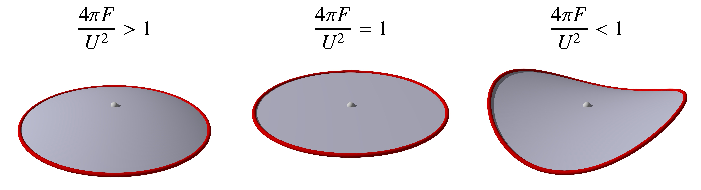
\includegraphics{chapters/tikz/4pifu2.pdf}
\caption{Das Verhältnis von Flächeninhalt zu Umfang im Quadrat einer
kleinen Kreisscheibe hängt von der Gausskrümmung ab. 
Für eine Flache Kreisscheibe gilt $4\pi F/U^2=1$ (Mitte).
Bei positiver Gausskrümmung (links) ist der Umfang gleich, der Flächeninhalt
aber grösser, daher wird das Verhältnis grösser.
Bei negativer Gausskrümmung (rechts) wird der Umfang deutlich länger, so dass
das Verhältnis kleiner wird.
\label{skript:kurven:4pifu2vis}}
\end{figure}
Dazu betrachten wir wieder eine Fläche der Form $z=f(x,y)$, deren
Tangentialebene im Nullpunkt die $x$-$y$-Ebene ist.
In dieser Fläche betrachten wir den Kreis parametrisiert mit
$x=R\cos t$ und $y=R\sin t$.
In einer Ebene wird der Flächeninhalt $F=\pi R^2$ sein, die Umfang $U=2\pi R$.
Man kann auch sagen, dass
\[
U^2 = 4\pi F
\qquad\Rightarrow\qquad
\frac{4\pi F}{U^2}=1
\]
ist.
Wir untersuchen, wie sich diese Beziehung ändert, wenn die
Fläche nicht mehr eine Ebene ist (Abbildung~\ref{skript:kurven:2pifu2vis}).

Wir approximieren die Fläche wieder als quadratische Funktion.
Zur Vereinfachung der Rechnung verwenden wir dabei ein Koordinatensystem,
in dem die Hauptrkümmungsrichtungen die Achsen sind.
Die Funktion $f(x,y)$ hat daher die Form
\[
f(x,y)
=
\kappa_1 x^2 + \kappa_2 y^2
\qquad\text{und}\qquad
g(x,y)=\begin{pmatrix}x\\y\\\kappa_1x^2 + \kappa_2y^2\end{pmatrix}.
\]
Für diese Fläche berechnen wir jetzt Flächeninhalt $F$ und 
Umfang $U$.

\subsubsection{Flächeninhalt}
Der Flächeninhalt einer mit $(u,v)$ parametrisierten Fläche $g(u,v)$
wird mit dem Integral
\[
F
=
\int_{D}
\biggr|\frac{\partial g}{\partial u} \times \frac{\partial g}{\partial v}\biggr|
\,du\,dv
\]
über das Definitionsgebiet $D$ der Fläche berechnet.
In unserem Fall verwenden wir $x$ und $y$ als Parameter und das
Definitionsgebiet
\[
D_R = \{ (x,y)\;|\; x^2 + y^2 < R\}.
\]
Der Betrag des Vektorprodukts im Integranden ist in unserem Fall
\begin{align*}
\biggl|
\frac{\partial g}{\partial x}
\times
\frac{\partial g}{\partial y}
\biggr|
&=
\left|
\begin{pmatrix}1\\0\\\frac{\partial f}{\partial x}\end{pmatrix}
\times
\begin{pmatrix}0\\1\\\frac{\partial f}{\partial y}\end{pmatrix}
\right|
=
\left|
\begin{pmatrix}1\\0\\2\kappa_1 x\end{pmatrix}
\times
\begin{pmatrix}0\\1\\2\kappa_2 y\end{pmatrix}
\right|
=
\left|
\begin{pmatrix}-2\kappa_1 x\\-2\kappa_2 y\\1
\end{pmatrix}
\right|
\\
&=
1 + 4\kappa_1^2 x^2 + 4 \kappa_2^2 y^2.
\end{align*}
Da das Integrationsgebiet eine Kreisscheibe mit Radius $R$ ist, verwenden
wir mit Vorteil Polarkoordinaten.
Wir ersetzen $x=r\cos\varphi$, $y=r\sin\varphi$ und $dx\,dy = r\,dr\,d\varphi$
und schreiben das Integral als
\begin{align*}
F
&=
\int_0^{2\pi}
\int_0^R
\sqrt{1 + 4\kappa_1^2 r^2 \cos^2 \varphi + 4\kappa_2^2 r^2\sin^2\varphi}
\,
r\,dr\,d\varphi
\end{align*}
Der Integrand ist leider zu kompliziert, um das Integral in geschlossener
Form derart auszuwerten, dass wir daraus die beabsichtigten Schlüsse
ziehen können.
Da wir aber schon bei der Funktion $f(x,y)$ nur mit einer Approximation
für kleine Werte von $r$ arbeiten, können wir den Integranden in eine
Taylorreihe in $r$ entwickeln.
Die Rechnung mit dem Maxima Programm
\lstinputlisting[style=Maxima]{chapters/listings/flaecheninhalt.maxima}
ergibt
\begin{align*}
F
%&=
%\int_0^{2\pi}
%\int_0^R
%\frac12R^2(1+R^2\kappa_1^2 \cos^2\varphi + R^2 \kappa_2^2\sin^2\varphi)
%\,r\,dr\,d\varphi
%\\
&=
\pi R^2
\bigl(
1
+
{\textstyle\frac12} R^2(\kappa_1^2+\kappa_2^2)
\bigr).
\end{align*}
Der erste Terme ist natürlich exakt der Flächeninhalt einer Kreisscheibe
in der Ebene.

\subsubsection{Umfang}
Für den Umfang berechnen wir das Wegintegral entlang des Randes.
Um eine Parametrisierung der Randkurve zu bekommen,
ersetzen wir $x=R\cos t$ und $y=R\sin t$ in $g(x,y)$ und erhalten
\[
c(t)
=
\begin{pmatrix}
R\cos t\\ R\sin t\\ R^2(\kappa_1^2\cos^2 t + \kappa_2^2\sin^2 t)
\end{pmatrix}
=
R
\begin{pmatrix}
\cos t\\ \sin t\\ R(\kappa_1^2\cos^2 t + \kappa_2^2\sin^2 t)
\end{pmatrix}
\]
Wir müssen den Betrag der Ableitung $\dot c(t)$ integrieren.
Das ist das Integral
\begin{align*}
U
&=
R
\int_0^{2\pi}
\sqrt{
\sin^2 t + \cos^2 t 
+ R^2(\kappa_1^2 \cos^2 t + \kappa_2^2\sin^2 t)
}
\,dt,
\end{align*}
welches sich ebenfalls nicht in geschlossener Form auswerten lässt.
Auch hier wählen wir wieder die Entwicklung in eine Taylorreihe nach $R$,
denn wir brauchen $U$ ja nur für kleine Werte von $R$.
Die Rechnung mit dem Maxima Programm
\lstinputlisting[style=Maxima]{chapters/listings/umfang.maxima}
gibt wieder
\begin{align}
U
&\simeq
R
\int_0^{2\pi}
1 + 2(\kappa_1^2 - 2\kappa_1\kappa_2 + \kappa_2^2)R^2 \cos^2 t\sin^2 t
\,dt
\notag
\\
&=
2\pi R
(
1
+ 
{\textstyle \frac14}(\kappa_1^2 -2\kappa_1\kappa_2+\kappa_2^2) R^2
).
\label{skript:kurven:U1}
\end{align}
Für die Beziehung zwischen Umfang und Flächeninhalt brauchen wir aber nicht
$U$ sondern sein Quadrat (auch dies wird im oben gelisteten Programm bereits
berechnet).
In unserer Näherung brauchen wir dabei nur Terme bis zur vierten Ordnung
in $R$ zu berücksichtigen.
Wegen $(1+x)^2 \simeq 1+2x$ in niedrigster Ordnung, bedeutet das nur,
dass wir den Term zweiten Term in der Klammer in \eqref{skript:kurven:U1}
verdoppeln müssen.
Wir bekommen daher
\begin{align*}
U^2
&\simeq
4\pi^2 R^2(
1
+
{\textstyle \frac12}
(\kappa_1^2-2\kappa_1\kappa_2 + \kappa_2^2)R^2
)
\end{align*}
als Approximation in niedrigster Ordnung.

\subsubsection{Beziehung zwischen Umfang und Flächeninhalt}
Wir müssen die Grösse $4\pi F/U^2$ untersuchen.
Mit den bisher berechneten Ausdrücken für $F$ und $U$ erhalten wir
\begin{align}
\frac{4\pi F}{U^2}
&=
\frac{4\pi^2R^2(1+{\textstyle\frac12}(\kappa_1^2 + \kappa_2^2)R^2)}%
{4\pi^2 R^2(1+{\textstyle\frac12}(\kappa_1^2-2\kappa_1\kappa_2+\kappa_2^2)R^2)}
=
\frac{1+(\kappa_1^2 + \kappa_2^2)R^2}%
{1+(\kappa_1^2-2\kappa_1\kappa_2+\kappa_2^2)R^2}.
\label{skript:kurven:4piu2}
\end{align}
Wieder brauchen wir nur eine Taylorreihe bis zur zweiten Ordnung in $R$.
Mit Hilfe der geometrischen Reihe 
\[
\frac1{1+x}= 1-x+x^2-x^3+\dots
\]
können wir den Nenner in~\eqref{skript:kurven:4piu2} in den Zähler
bringen.
Wenn wir wieder Terme höherer Ordnung als $R^2$ weglassen, bekommen
wir 
\begin{equation}
\frac{4\pi F}{U^2}
\simeq
1+\kappa_1\kappa_2R^2
=
1 + KR^2
\end{equation}
als Schlussresultat.
Das Produkt der Hauptkrümmungen ist die Gausskrümmung $K=\kappa_1\kappa_2$,
diese beschreibt also im Wesentlichen das Anwachsen des Verhältnisses
von Flächeninhalt zu Umfang im Quadrat eines Kreises in Abhängigkeit
von dessen Radius.
Bei positiver Gausskrümmung wächst das Verhältnis schneller an
als auf einer Ebene, bei negativer Gausskrümmung langsamer.





